 In the SM the flavour structure is encoded in 
 the Higgs couplings to the fermions. 
 
\textbf{ Fermion masses.} In the SM the  
diagonalized Yukawa couplings, $y_f$, are
proportional to the fermion masses, $m_f$,  with a common
factor,  $y_f = \sqrt{2} \kappa_f m_f / v$, where  $\kappa_f^{\rm SM}=1$;
moreover,
there are no tree-level flavour changing couplings of the Higgs. This may change in the presence of new physics, in which case the couplings of the Higgs to the fermions can in general take the form, $\mathcal{L}_{\rm eff} = -\kappa_{f_i} (m_{f_i}/{v}) h \bar f_i f_i + i \tilde \kappa_{f_i} (m_{f_i}/v) h \bar f_i \gamma_5 f_i  
	- \big[\big( \kappa_{f_i f_j} + i \tilde \kappa_{f_i f_j} \big) h \bar f_L^i f_R^j +{\rm h.c.}\big]_{i\neq j}. $
	Currently, only the third generation Yukawa couplings have been measured, having been found to be in agreement with the SM predictions, while for the Higgs couplings to the first two generations, only upper bounds exist. 
Experimentally, a number of SM predictions for the Higgs couplings to fermions 
must be tested as precisely as possible: {\em (i)} proportionality, $y_f\propto m_f$; {\em (ii)} the factor of proportionality, $\kappa_{f_i}=1$; {\em (iii)} diagonality (no off-diagonal flavour violating couplings at tree level, $\kappa_{f_i f_j}=\tilde \kappa_{f_i f_j}= 0$); {\em (iv)} reality (no CP violation at tree level, $\tilde \kappa_{f_i}=\tilde \kappa_{f_i f_j}=0$) \cite{Nir:2016zkd}.

\begin{figure}[t]
	\centering
	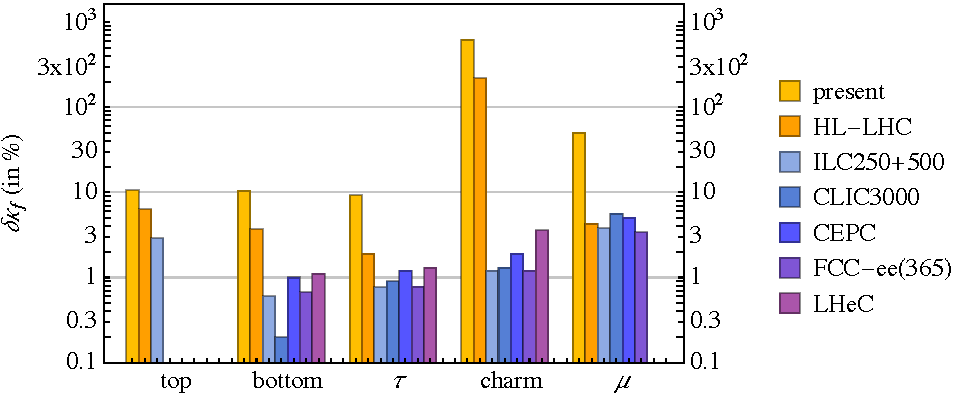
\includegraphics[width=0.75\textwidth]{\main/Flavour/figs/kappaplot}\vspace*{3mm}\\
       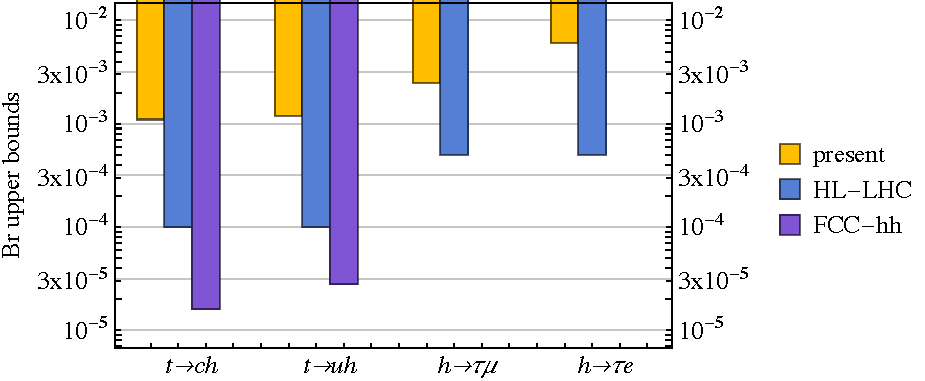
\includegraphics[width=0.75\textwidth]{\main/Flavour/figs/BrplotFV}
	\caption{Summary of the  projections for measurements of Higgs Yukawa couplings to quarks and leptons (upper panel), and on select flavour violating decays (lower panel), adapted from Ref.~\cite{Heinemann:2019trx}. 
	\label{fig:higgs:forecast}}
\end{figure}
The summary of the expected experimental sensitivies is shown in Fig.~\ref{fig:higgs:forecast} (upper panel) using the $\kappa_f$ framework as a toy approximation to show sensitivity in each channel (a global view of experimental constraints using SM-EFT can be found in \cite{deBlas:2019rxi}). 
The sensitivity in the muon channel is now close to what is required to test the SM prediction for the muon Yukawa. This will be the first meaningful test of the 2nd generation Yukawa couplings. A precision measurement does require larger datasets that will be provided in the {\bf short- and mid-term} by the LHC in Run 3 and by the \HLLHC.
In the {\bf mid-term}, the \HLLHC will bound the Yukawa couplings to the third generation fermions and to the muon to a few percent level. 
In the {\bf long-term}, the proposed large scale experiments, \ILC, \FCCee, \CEPC, and \CLIC can significantly improve this precision, to below percent level. They would also measure the charm Yukawa coupling for the first time, and probe it quite precisely, at the percent level. A slightly more modest improvement can be expected at the \HELHC \cite{deBlas:2019rxi}. 
In addition, at \FCCee the upper bound of $\delta y_e/y_e<1.6$ can be achieved after
one year of running at $\sqrt{s}=m_h$. 

\textbf{ Flavour violating Higgs decays}: for the branching ratios of $h\to \tau\mu, \tau e$ decays,  in the {\bf mid-term}  \HLLHC is expected to improve the reach by an order of magnitude, to the level of $5\times 10^{-4}$, see Fig.~\ref{fig:higgs:forecast} (lower panel).  
Figure~\ref{fig:NPscales} illustrates in light (dark) red the scale reach of present data (\HLLHC prospects). Taking $h\to \mu\mu$ and $h\to \tau\tau$ as guidance, one can expect {\bf in the long term} another one to two orders of magnitude improvements for $h\to \tau\mu$ at \FCChh \cite{deBlas:2019rxi}.


\textbf{The top quark} is unique among the SM fermions, with its ${\mathcal O}(1)$ coupling to the Higgs. Such a large Yukawa coupling for the top is also the origin of the weak scale hierarchy problem -- the quadratically divergent corrections to the Higgs mass are a problem precisely because of it. 
It is thus very common for new physics models that address the  hierarchy problem to also lead to modifications of the top quark properties.  
Studying precisely the latter may in addition give insight into the origin of the SM flavour puzzle, or at least as to why one and only one Yukawa coupling is large.  Experimentally, new physics is probed using FCNC top decays, $t\to c\gamma, cZ, cg, ch$. 
The present upper bounds on their branching ratios are in the range $10^{-3}-10^{-4}$, and will be improved by an order of magnitude or more in the {\bf mid-term} at \HLLHC, resulting in about a two-fold increase in the reach to the effective new physics scale, cf. Fig. \ref{fig:NPscales}.
Also in the mid-term, the reach for  $t\to hc, hu$ decays is expected to improve  by one order of magnitude from the present $10^{-3}$ level,   at \HLLHC; see Fig.~\ref{fig:NPscales} (dark red) for the corresponding sensitivity to new physics scales. This is expected to be further improved in the {\bf long-term}  at \FCChh, see Fig.~\ref{fig:higgs:forecast} (lower panel).

\textbf{The $Z$ boson} is also a sensitive probe of new physics: for instance, the observation of flavour violating $Z\to e\mu, \mu\tau, e\tau$ decays would be a clear evidence of new physics, for instance, the existence of sterile neutral fermions. The current limits on these decays are ${\mathcal O}(10^{-6}-10^{-5})$, and could be improved by several orders of magnitude, down to ${\mathcal O}(10^{-9})$ at \FCCee \cite{Abada:2019lih}. 


Lepton flavour violating transitions such as $e^+e^-\to e^+\tau^-$ would also probe \textbf{contact interactions}. The LFV operators of the schematic form $(\bar e e)(\bar e \tau)$ could be well probed at future high energy $e^+e^-$ colliders, and would increase the present bound of $\sim9$~TeV (on the scale of the contact interaction) to 35~TeV at a \CLIC running at 3~TeV~\cite{deBlas:2018mhx}. 


